%%%%%%%%%%%%%%%%%%%%%%%%%%%%%%%%%%%%%%%%%%%%%%%%%%%%%%%%%%%%    
\section{Data Exploration}
%\begin{}{2}
% \begin{shadequote}[r]{From the spec}        
% What you learned from your initial analysis of the data.
% \end{shadequote}

\subsection{World Data}
% \todo {Some suggestions.
% - Data by region. e.g. WorldMaps for data availability.
% - World map that indicates heat map for gap.}

Using the OECD data, we found out the top countries reporting worst GPG percentages in 2018. It must be noted that not all countries report their GPG and hence the plot in Figure \ref{fig:top-10-gpg} shows a partial story.

    \begin{centering}
        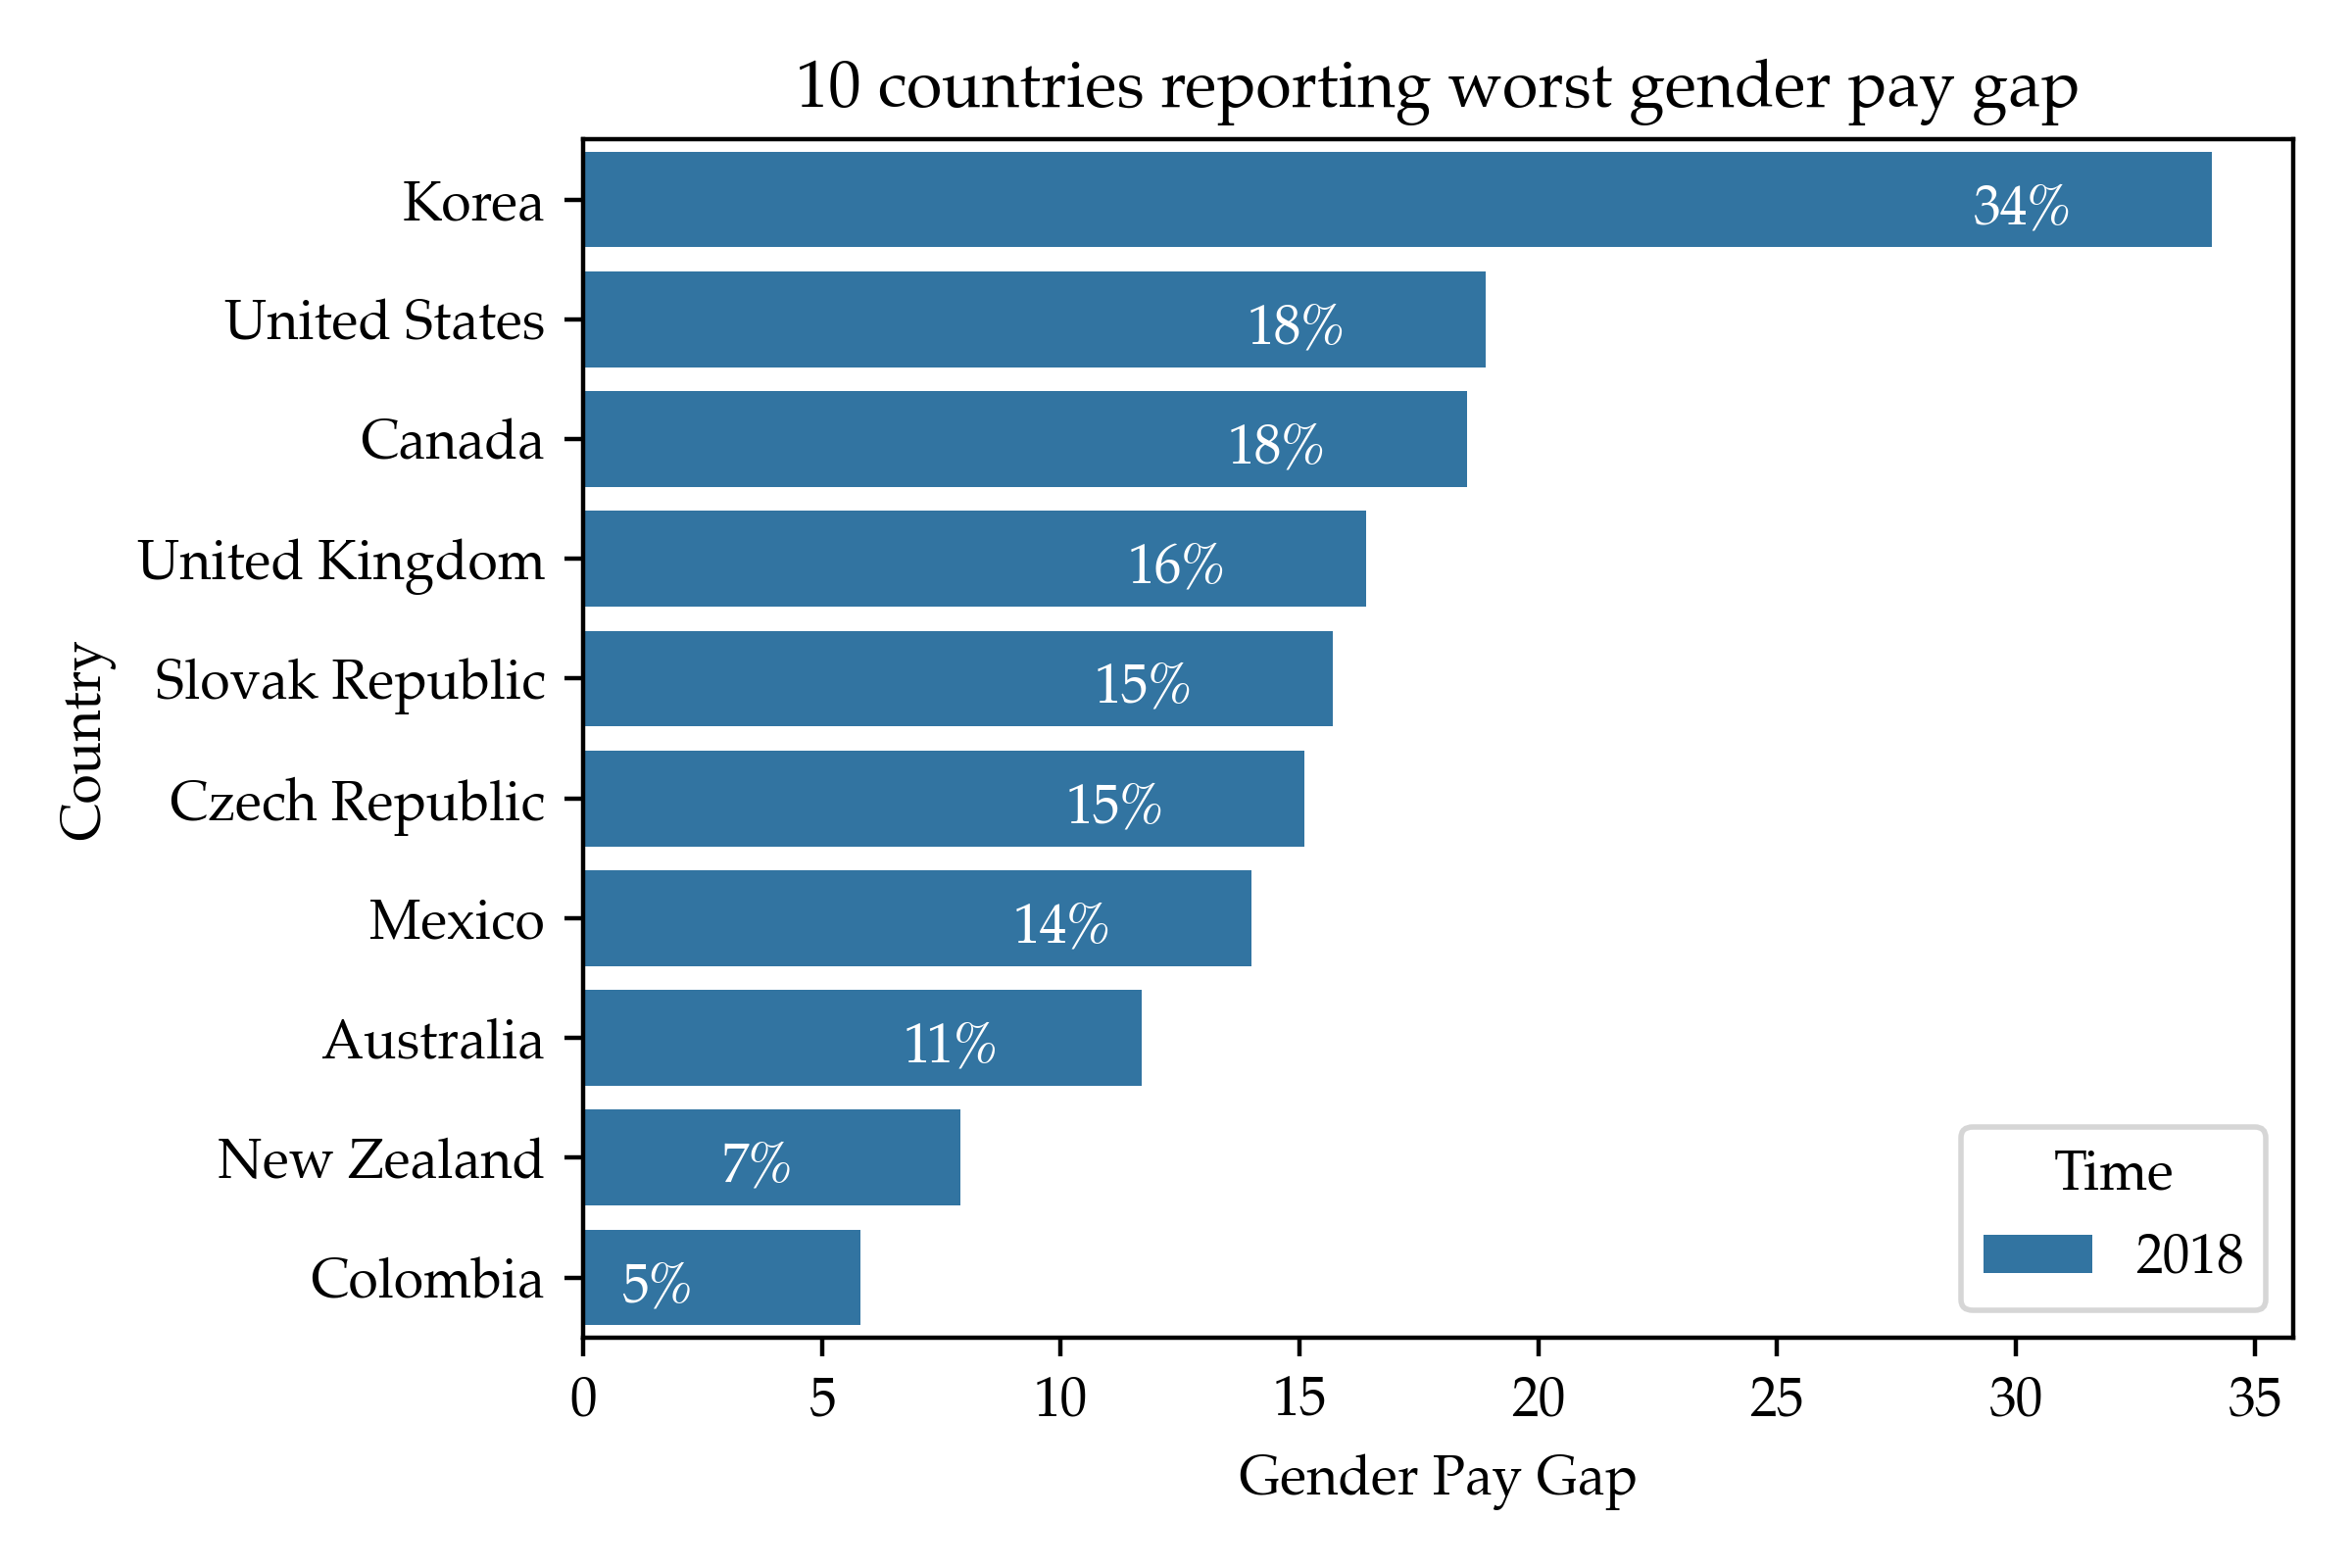
\includegraphics[width=0.99\linewidth]{images/Top10Countries.png}
        \captionof{figure}{Comparison of 10 OECD countries' GPG in 2018}
        \label{fig:top-10-gpg}
    \end{centering}
    
OECD data provided GPG percentages from 2000 to 2018 for the above countries and that was plotted to see the trend over the past 18 years in figure \ref{fig:country-time-gap}. A decrease in the pay gap can be observed from the graph for most countries. The decreasing trend is different for different countries that indicates an effect of different policies in place.

    \begin{centering}
        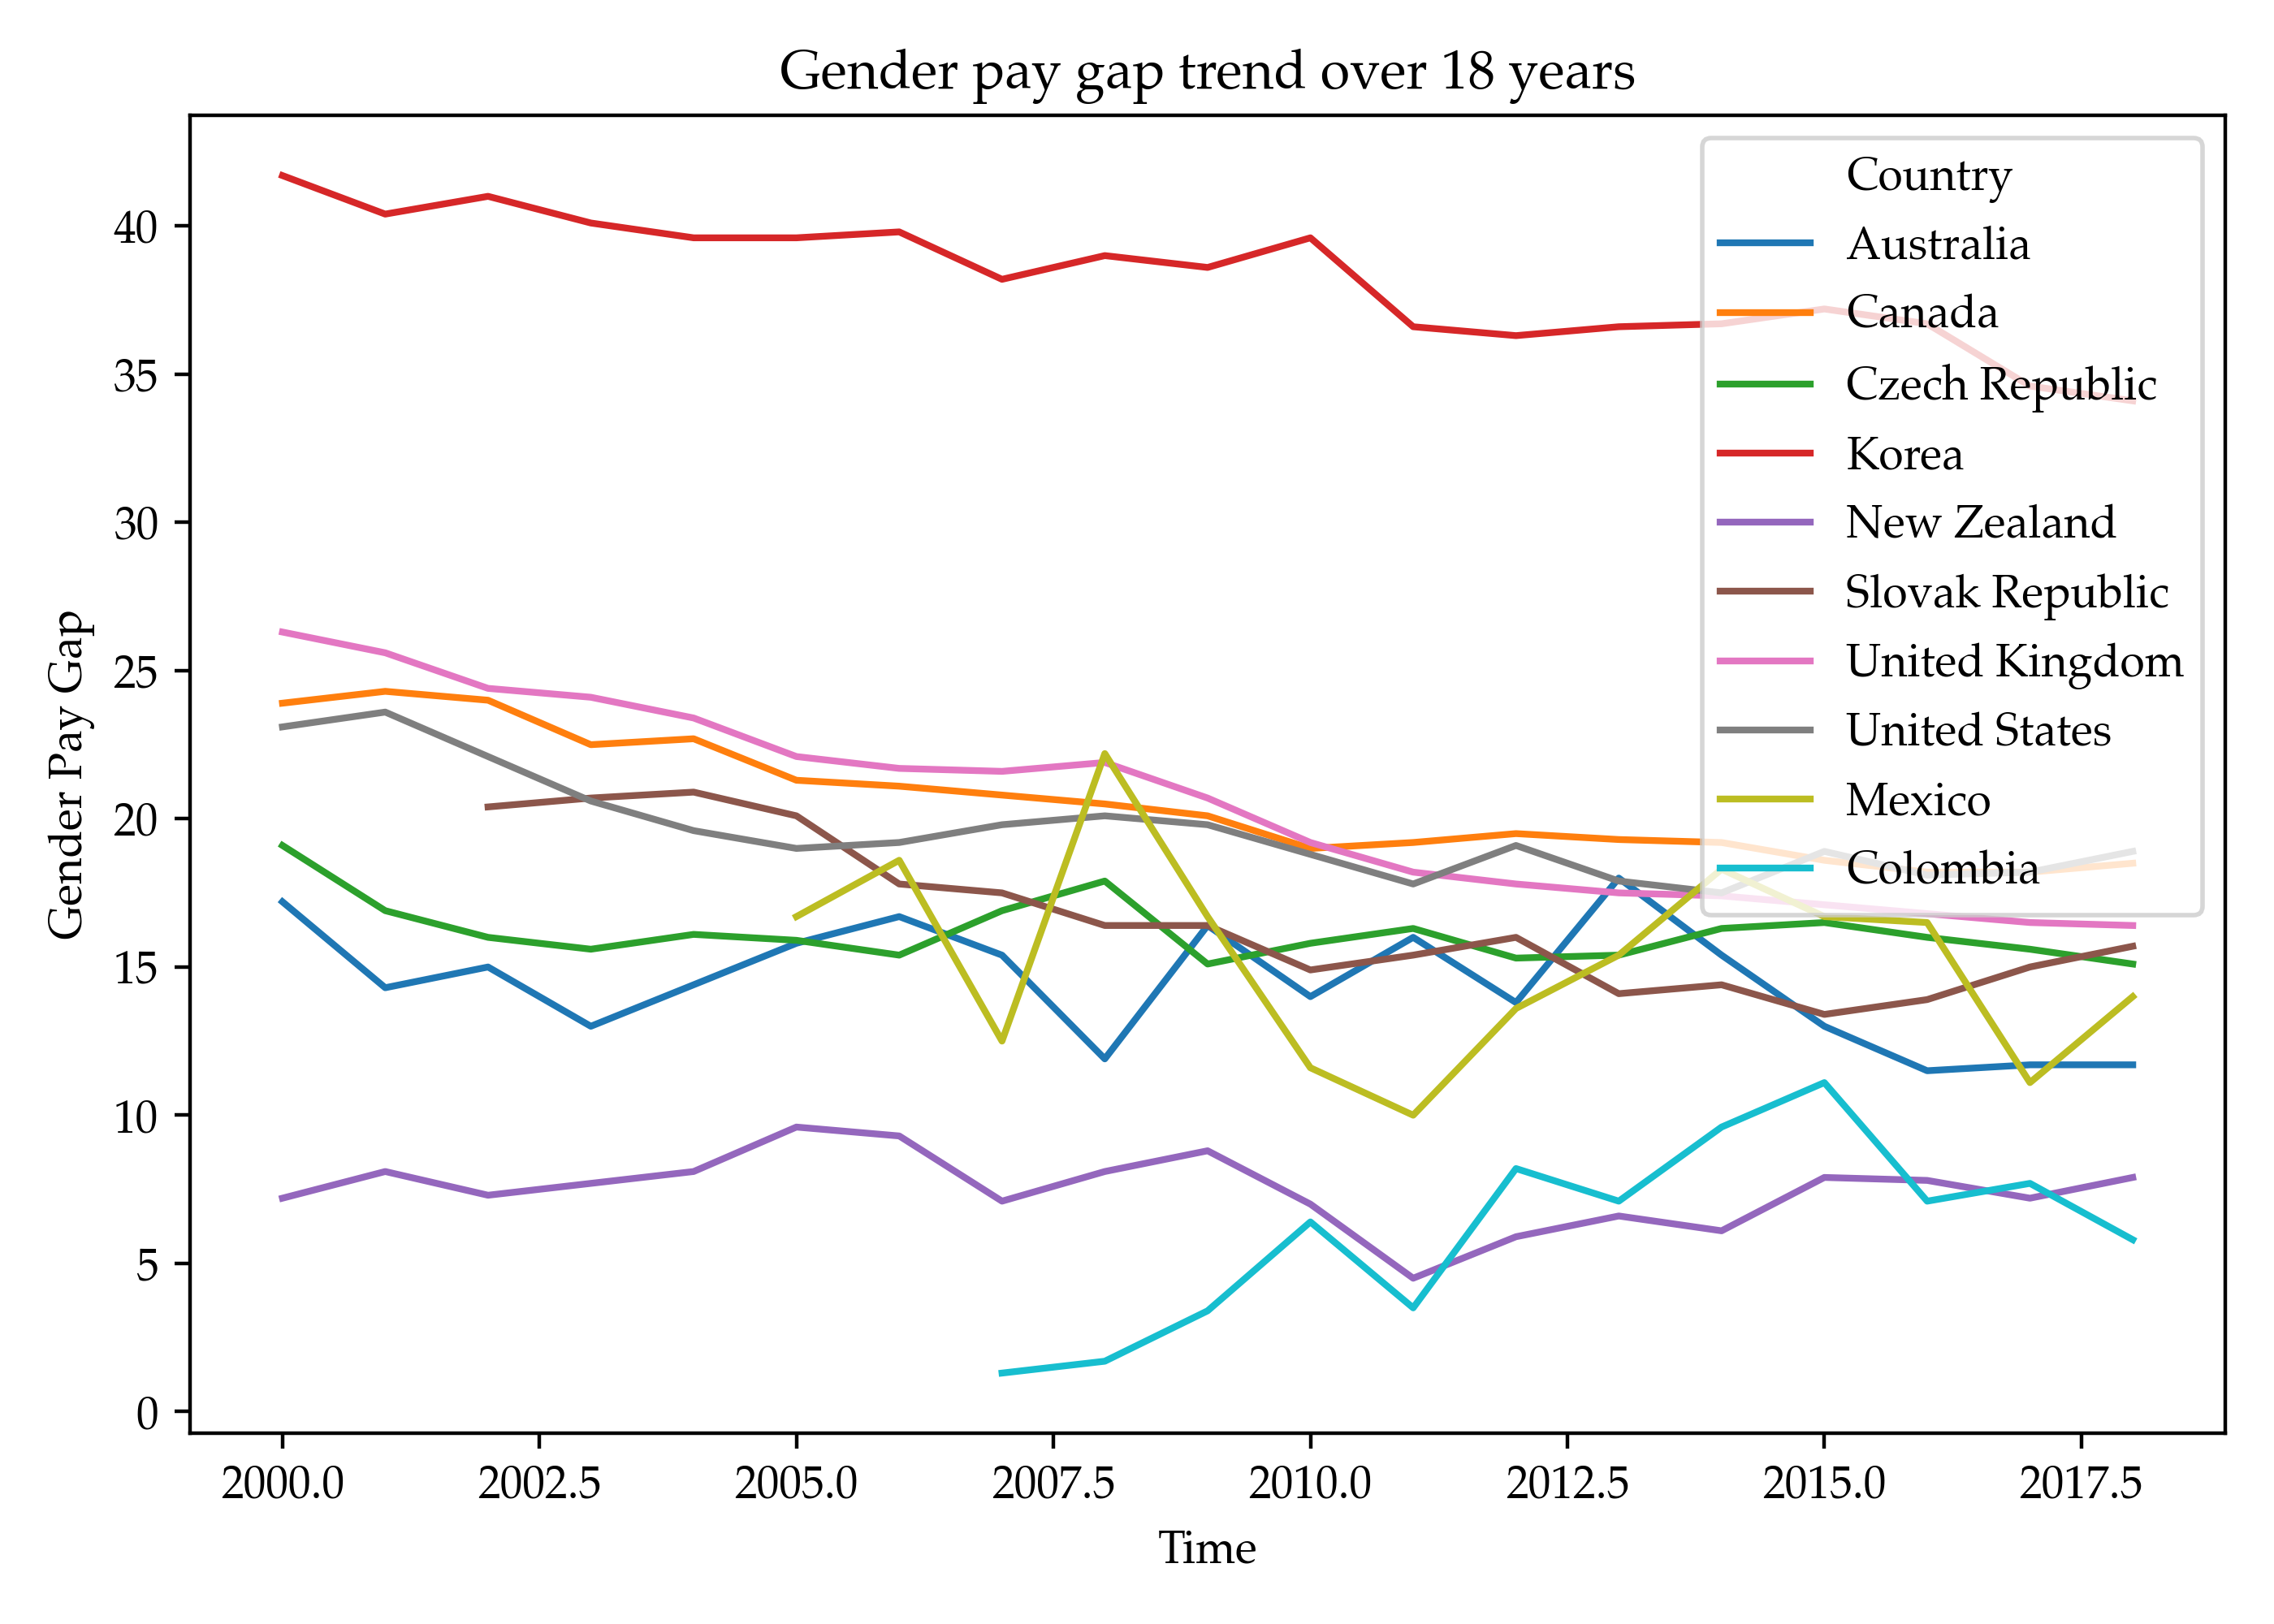
\includegraphics[width=0.99\linewidth]{images/Country_time.png}
        \captionof{figure}{The GPG over two decades for various OECD countries}
        \label{fig:country-time-gap}
    \end{centering}

\subsection{UK Data}

\paragraph{Company sizes}
    The companies are categorised by the number of employees in the data and a representation of the different percentage of companies in each category is shown in Figure \ref{fig:employer-size-dist}. We see an imbalance in the percentages which indicates that this feature will not be useful in modelling if we attempt to do a classification.

    \begin{centering}
        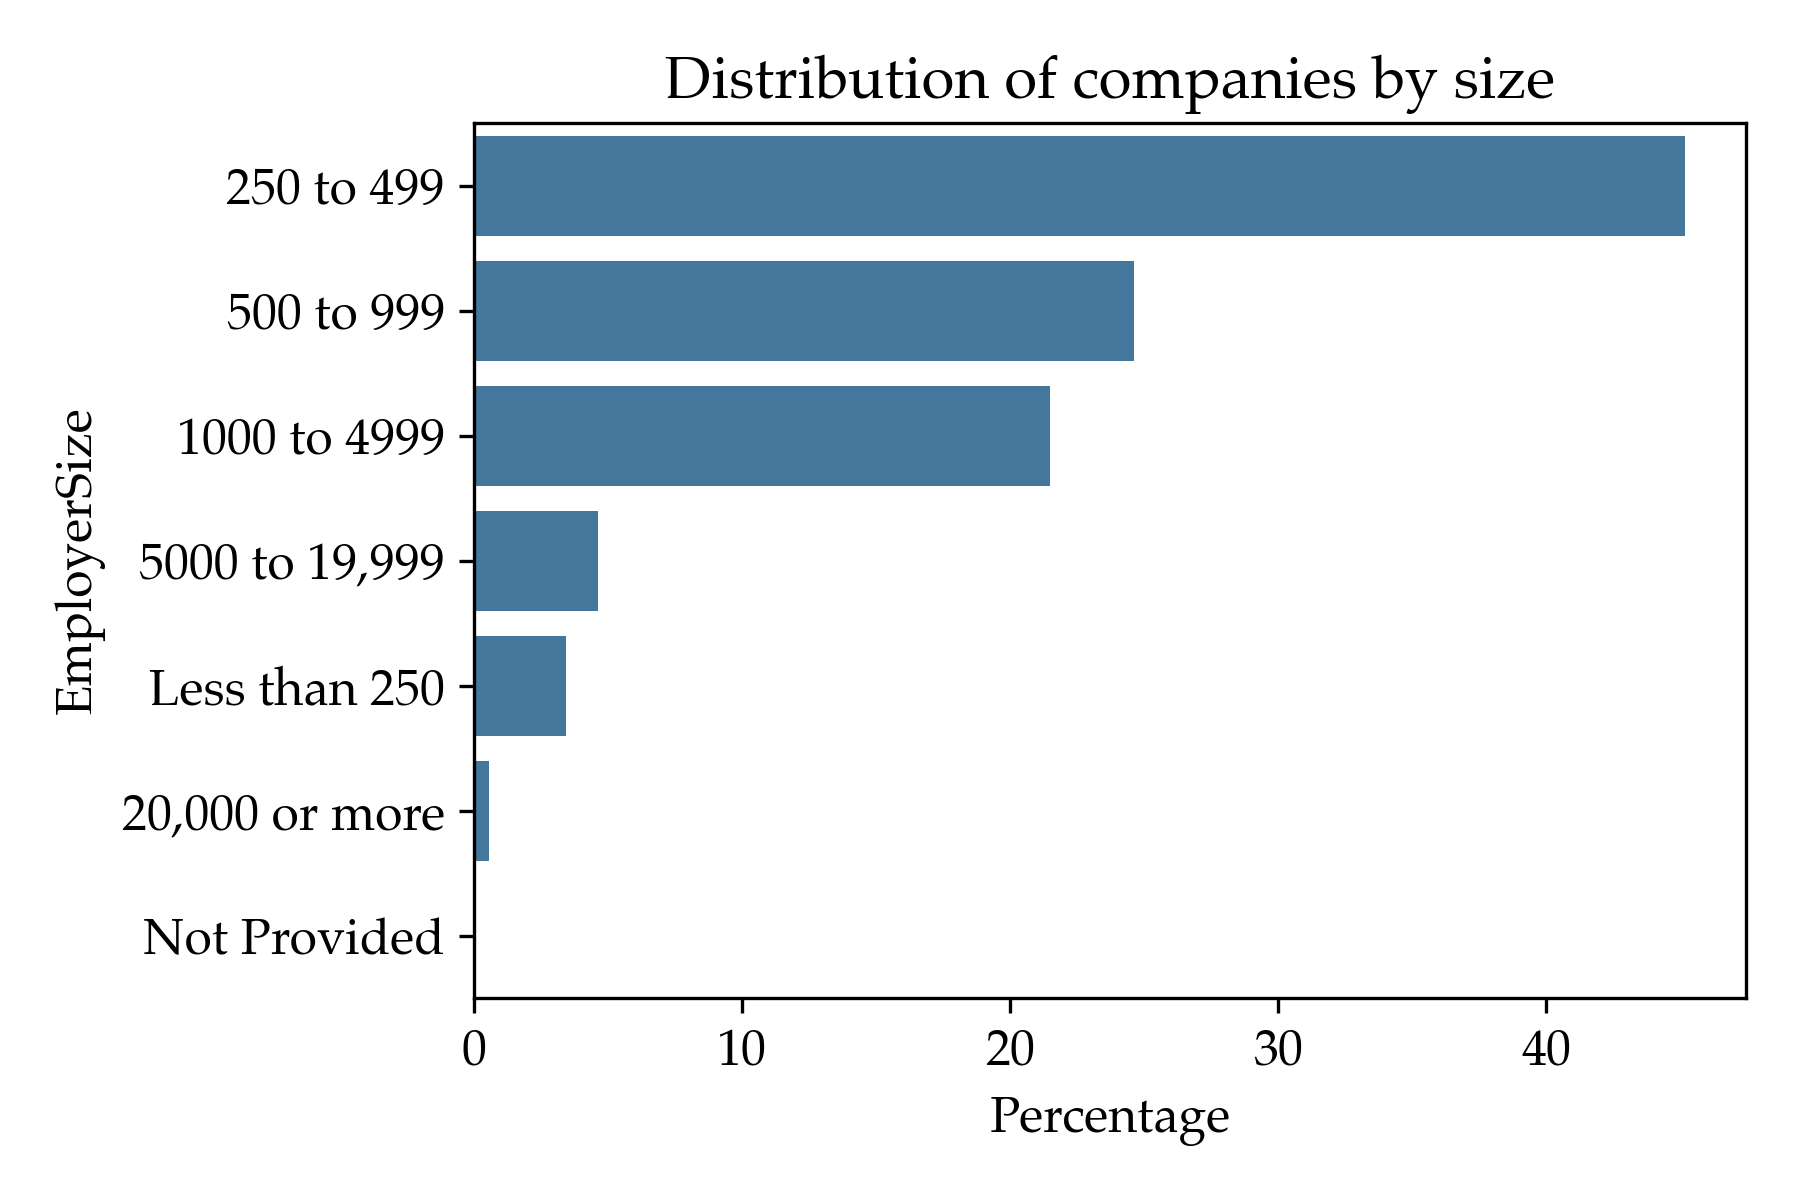
\includegraphics[width=0.9\linewidth]{images/EmployerSize2018.png}
        \captionof{figure}{\code{EmployerSize} distribution}
        \label{fig:employer-size-dist}
    \end{centering}

\paragraph{Companies grouped by Industrial Sector}
    The number of countries in each industrial sector (at top-level granularity) as shown in Figure\ \ref{fig:companies-by-sector}. Illustrates the general demographic of the data where the majority of the data arises from Education, Manufacturing and etc.

    \begin{centering}
        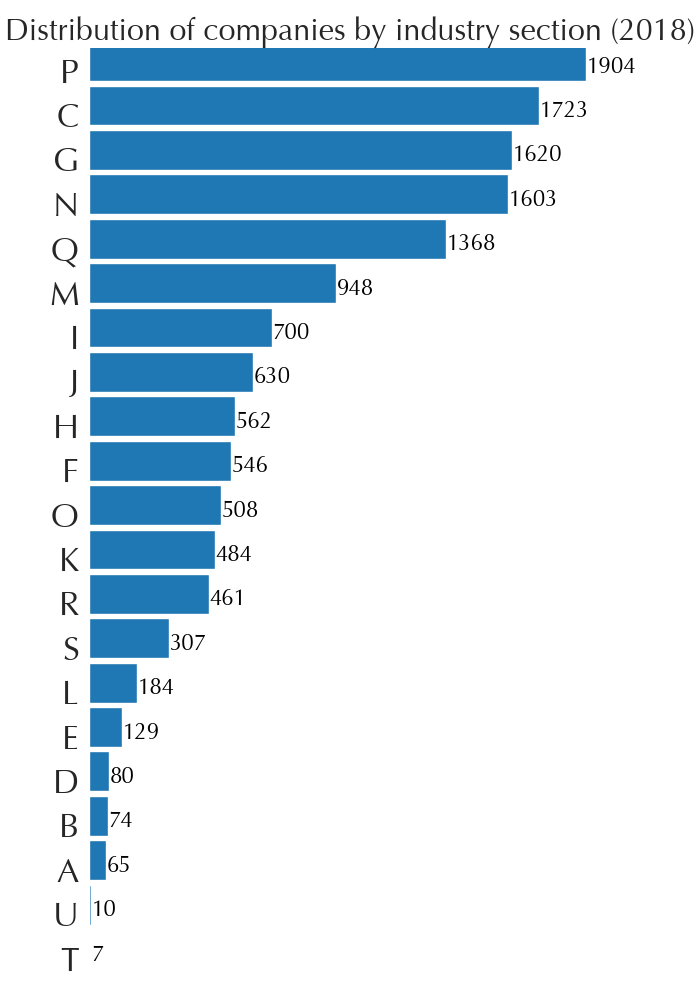
\includegraphics[width=0.6\linewidth]{images/2018-all-companies-sectors.png}
        \captionof{figure}{       \begin{scriptsize}Number of companies by section in 2018: the top 5 are (P): Education, {\bf (C):} Manufacturing, {\bf (G):} Wholesale and retail trade, {\bf (N):} Administrative and support service activities and {\bf (Q):} Human health and social work activities. The rest of the codes is listed in Appendix \ref{app:sector_codes}        \end{scriptsize} }
        \label{fig:companies-by-sector}
    \end{centering}
\vspace{-1.5em}
\paragraph*{Proportion of employees by gender}
The data includes the percentage of men and women in each pay quartile per company, so it is possible to determine the gender composition of each company's entire workforce by averaging the quartile representations for each gender. 


\begin{centering}
    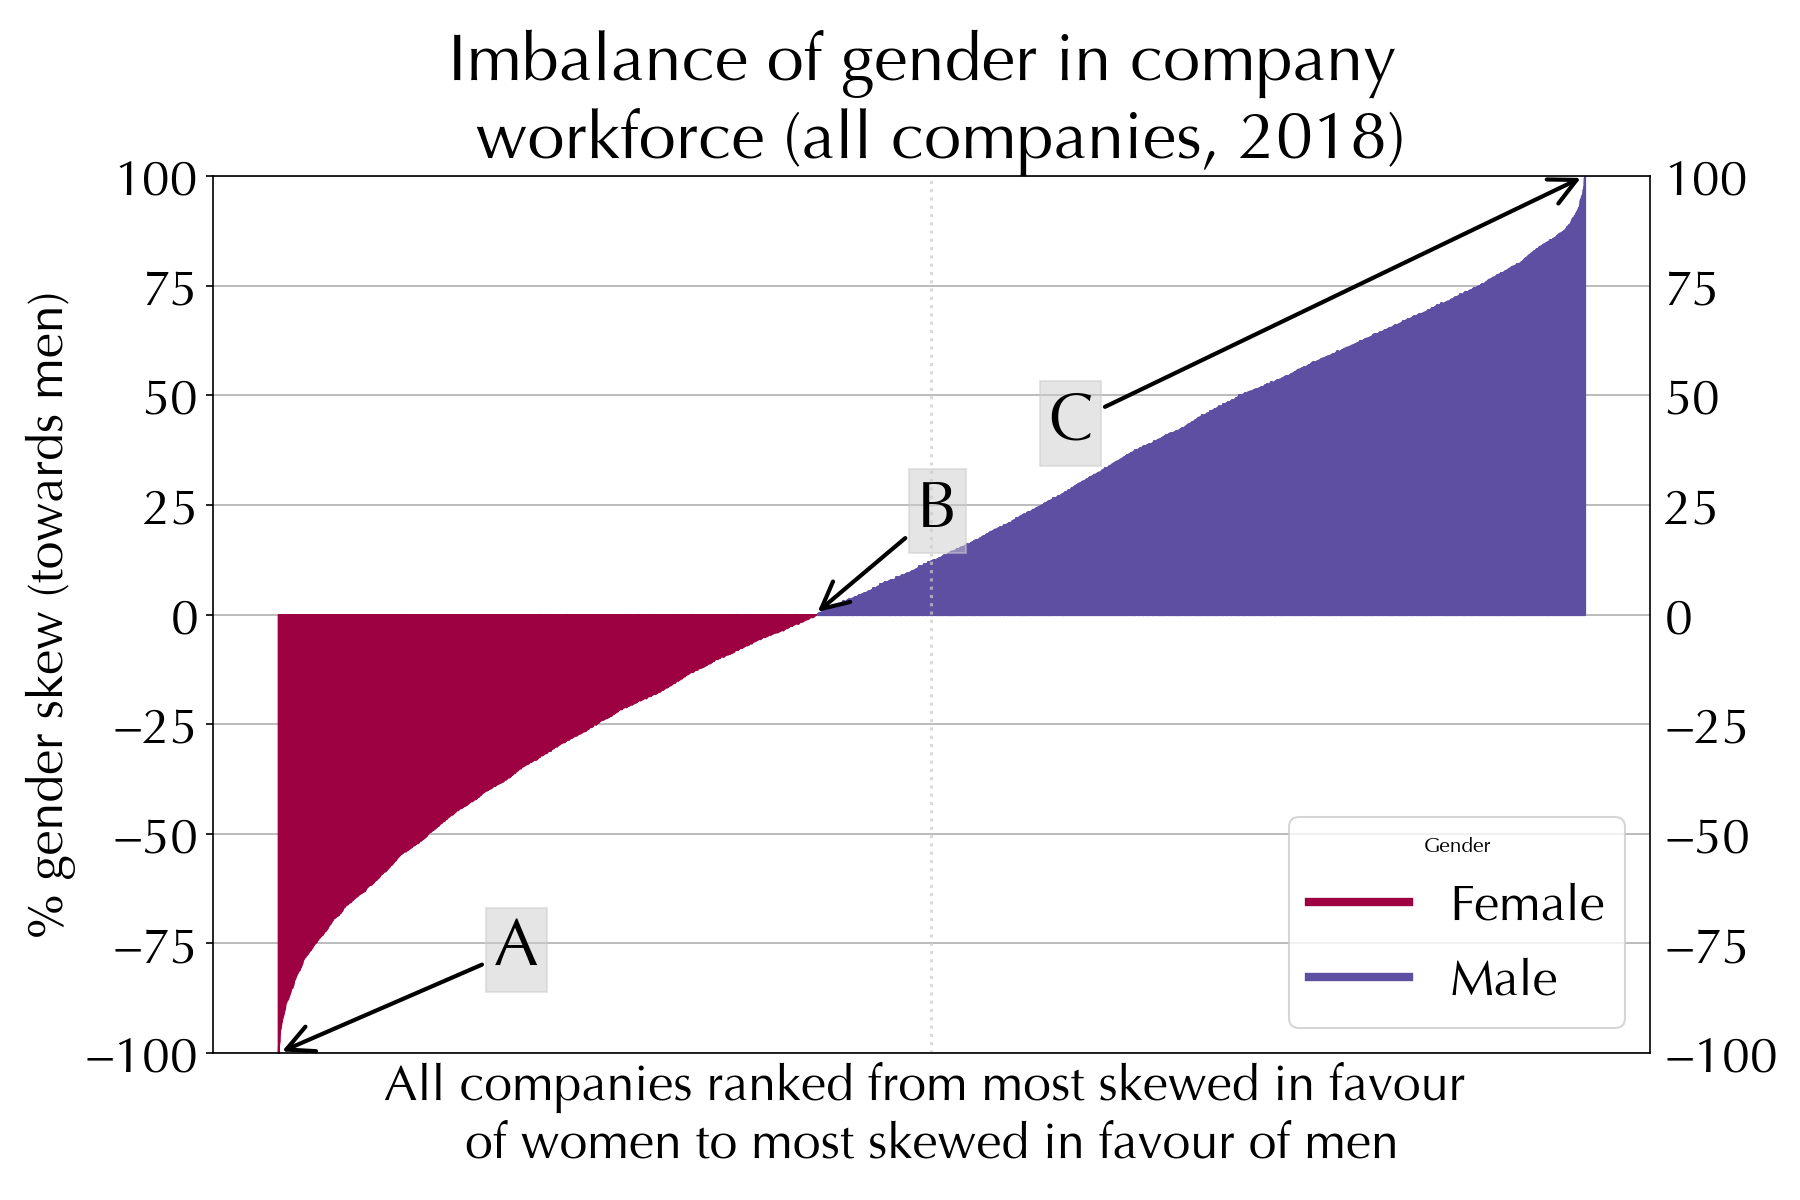
\includegraphics[width=\linewidth]{images/2018-all-companies-gender-makeup.png}
    \captionof{figure}{        \begin{scriptsize}Gender composition of all companies in 2018. Companies are ranked from left to right by their skew towards men. As can be seen from the relative widths of the blue and red areas, there are more companies which are predominantly male. At the extremes, there are companies which only have employees of the same gender.
        {\bf(A)} Most skewed towards women. At \emph{Additions (U.K.) Limited} there are 100\% more women than men
        {\bf(B)} Most equal representation. At \emph{Swinton (Holdings) Limited} there are equal numbers of men and women
        {\bf(C)} Most skewed towards men. At \emph{Speedy Transport Limited}  there are 100\% more men than women        \end{scriptsize}
    }
    \label{fig:workforce-composition}
\end{centering}
\justify

This is visualised in for 2018 in Figure \ref{fig:workforce-composition}. At the extremes, there are companies staffed entirely by men or entirely by women, but these are outliers. Overall, we see that a small majority of companies in the UK are predominantly staffed by men.

\paragraph{Mean vs Median pay gap}
    In Figure \ref{fig:DiffMedian-DiffMean relation} we show how the a general difference between median and mean of the hourly pay percentage to be fairly similar in both cases. But a more insightful representation is shown by Figure \ref{fig:lower-quartile} and \ref{fig:upper-quartile} looking into the upper and lower quartiles.

    \begin{centering}
        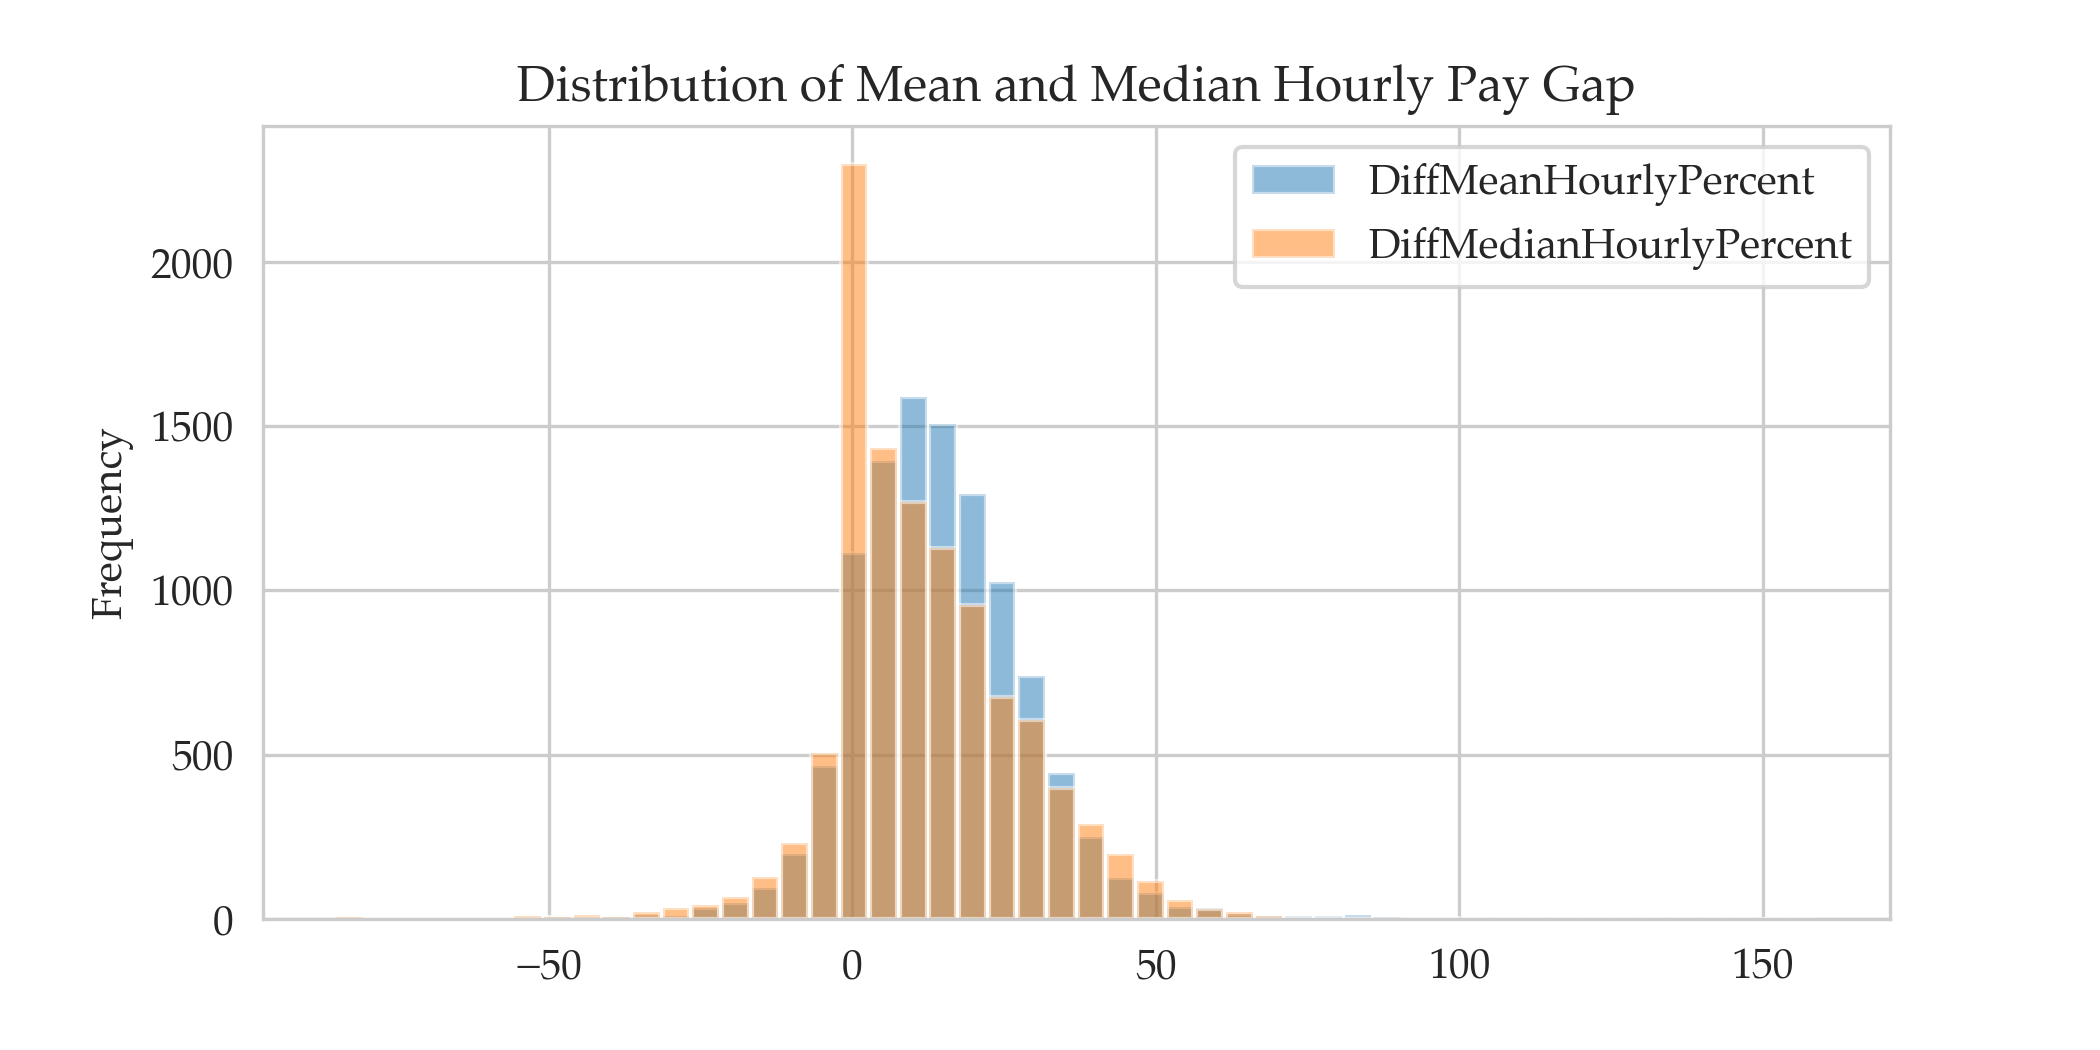
\includegraphics[width=1\linewidth, scale = 1.7]{images/diff_mean_vs_median.plot.png}
        \captionof{figure}{\begin{scriptsize}Histogram of \code{DiffMedian} and \code{DiffMean} relation distribution\end{scriptsize}}
        \label{fig:DiffMedian-DiffMean relation}
    \end{centering}
\vspace{-1.2em}    
\paragraph{Genders making up each pay quartile} 
Distribution of the percentages of each gender making up the various pay quartiles is shown in Figure \ref{fig:Distribution of GPG per quartile 2017}. The male and female proportions are duals, and so are symmetric.
    
        \begin{centering}
        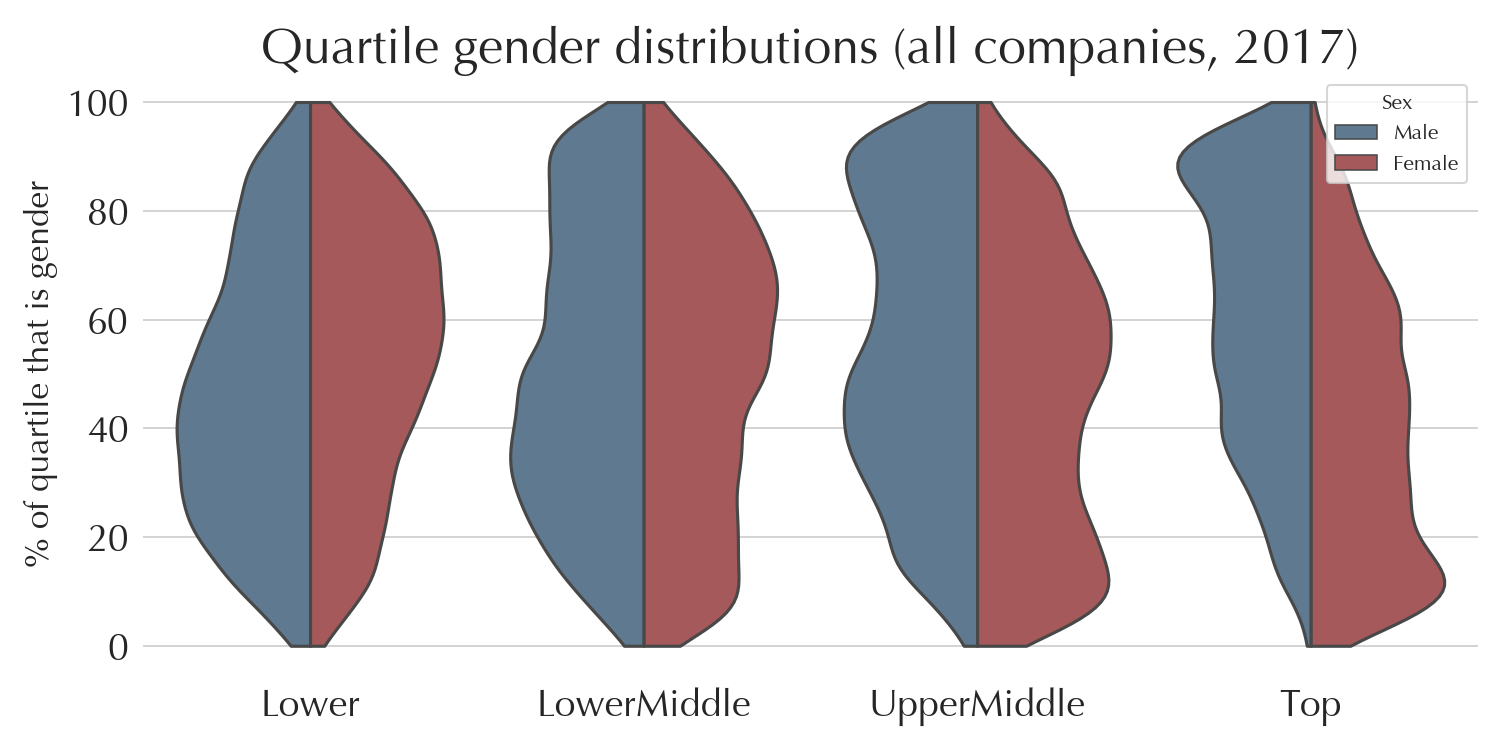
\includegraphics[width=0.99\linewidth]{images/2017-all-companies-quartiles.png}
        \captionof{figure}{Distribution of percentage GPG per quartile}
        \label{fig:Distribution of GPG per quartile 2017}
    \end{centering}
    We see that the situation is very unequal: men are much more likely to make up a big percentage of the top quartile and a small percentage of the lowest-paid quartile.
    
%      whereby the Lower and LowerMiddle region of violin plot illustrate a larger distribution of females to be found in this quartile compared to their male counterpart. 
% While the UpperMiddle shows a a bi-model distribution for both gender though the percentage of employee are found in the lower end with 58\% and 12\% compared to 92\% and 47\% of males. With the Top quartiles shows a large  of male employees in the top quartile of a company.   

\paragraph{Fairness of representation by gender in the top vs lowest pay quartiles}
  We derived additional indicators that compensate for the gender mix in a company. We try to ask the question \textit{What percentage of the company's women are in the top quartile?} rather than \textit{What percentage of the employees in the top quartile are women?} 
   
  The 2018 gender representation in the lower quartile is shown in Figure \ref{fig:lower-quartile} and for the upper
  quartile in Figure \ref{fig:upper-quartile}. Most companies have an over-representation of the male
  workforce in the top quartile and an over-representation of the
  female workforce in the bottom quartile, and our exploration of the data showed the trend holding for 2017 and 2019 as well.
   
    \begin{centering}

        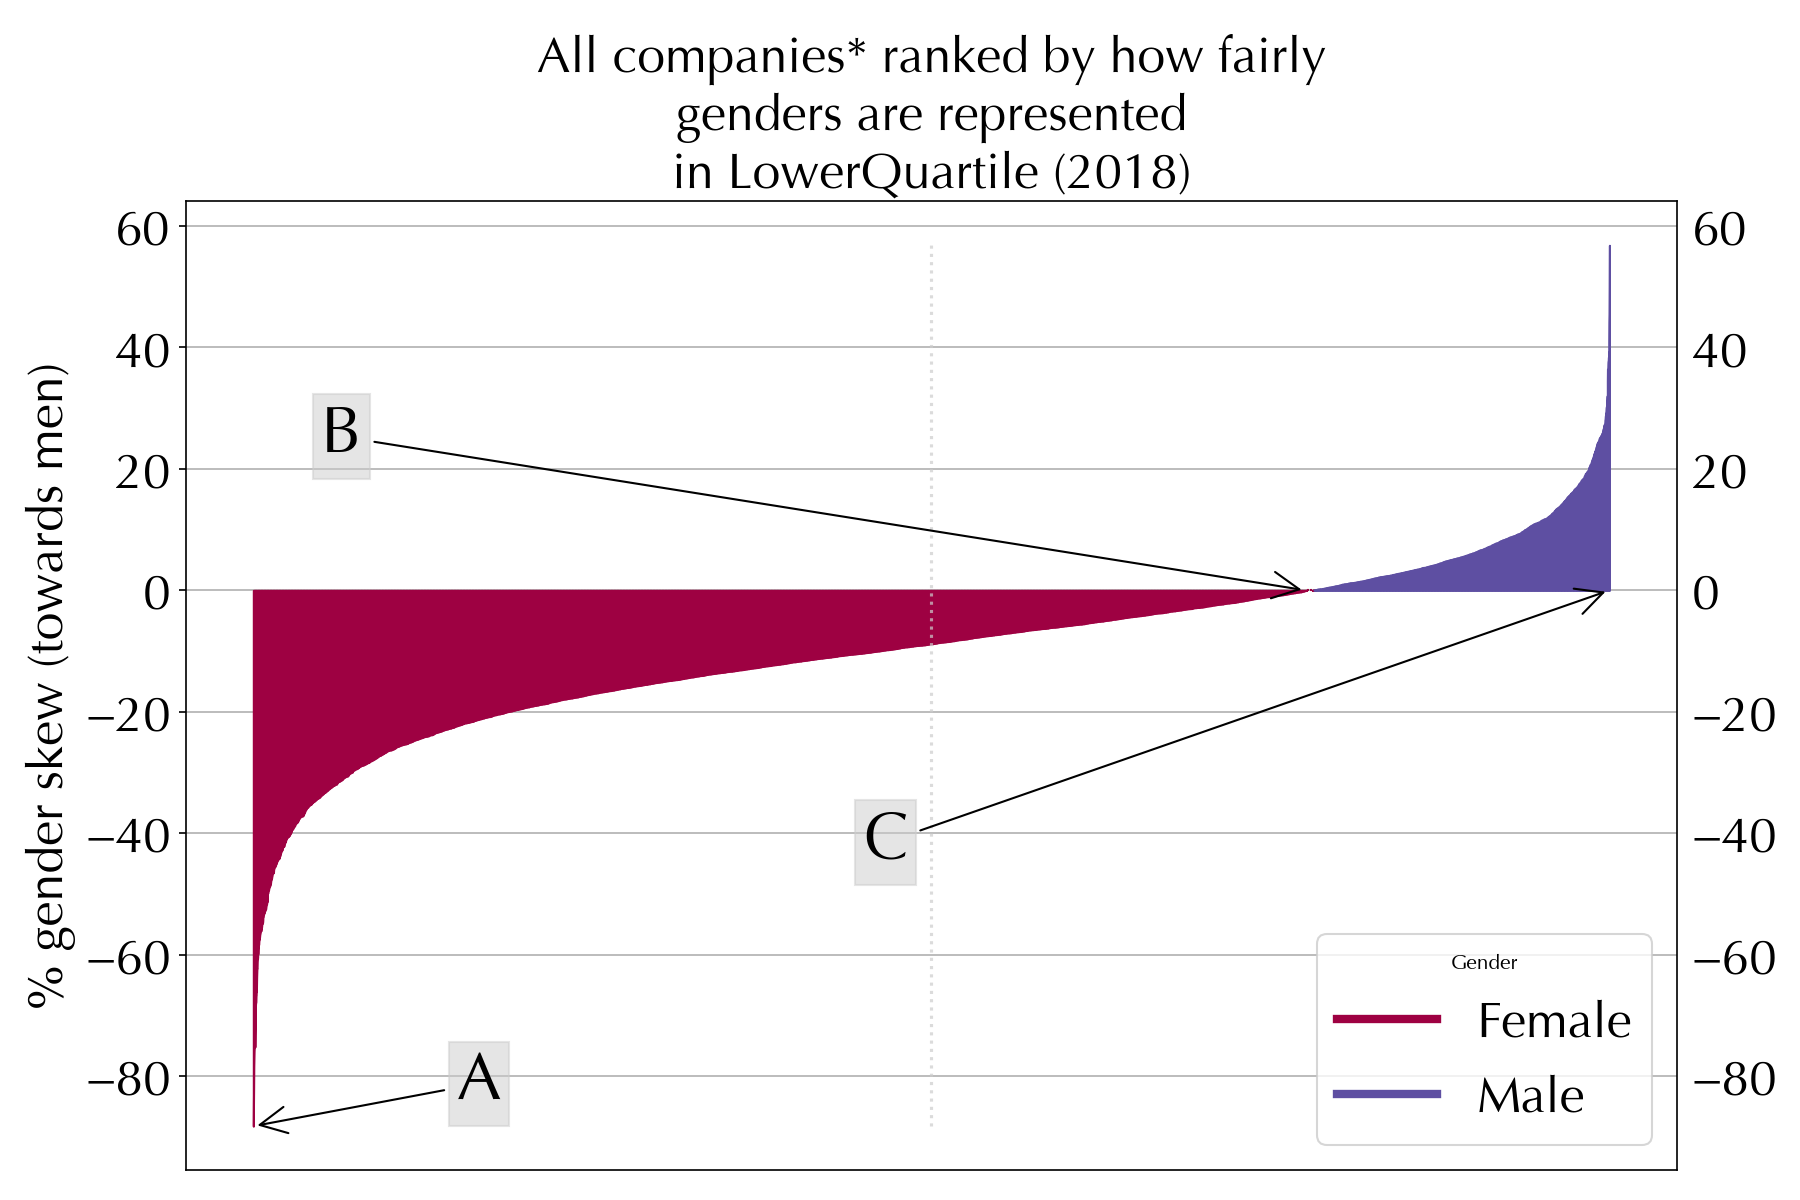
\includegraphics[width=\linewidth]{images/2018-how-fair-genders-LowerQuartile.png}
        \captionof{figure}{            \begin{scriptsize}
2018 Bottom quartile gender representation imbalance (only showing companies that had employees of both genders.) Companies are ranked by fairness of representation of gender in the quartile from most skewed towards women to most skewed towards men from left to right.  \textbf{(A):} Most skewed towards women: At \emph{Kongsberg Automotive Limited,} 100\% of the company's women are in the bottom quartile vs 11.8\%  of the company's men. 15\% of the employees are female.
            \textbf{(B):}  Most equal: At \emph{Coquet Trust}, 25\% of company's women are in the bottom quartile, vs 25\% of the company's men. 70\% of employee are female.  
            \textbf{(C):} Most shewed towards men: Most equal representation: At \emph{Maxim facilities Management Ltd.,} 11.2\% of the company's women are in the bottom quartile, vs 68\% of the company's men. 75.8\% of employee are female.
                  \end{scriptsize}  }

        
        \label{fig:lower-quartile}
    \end{centering}

    \begin{centering}
        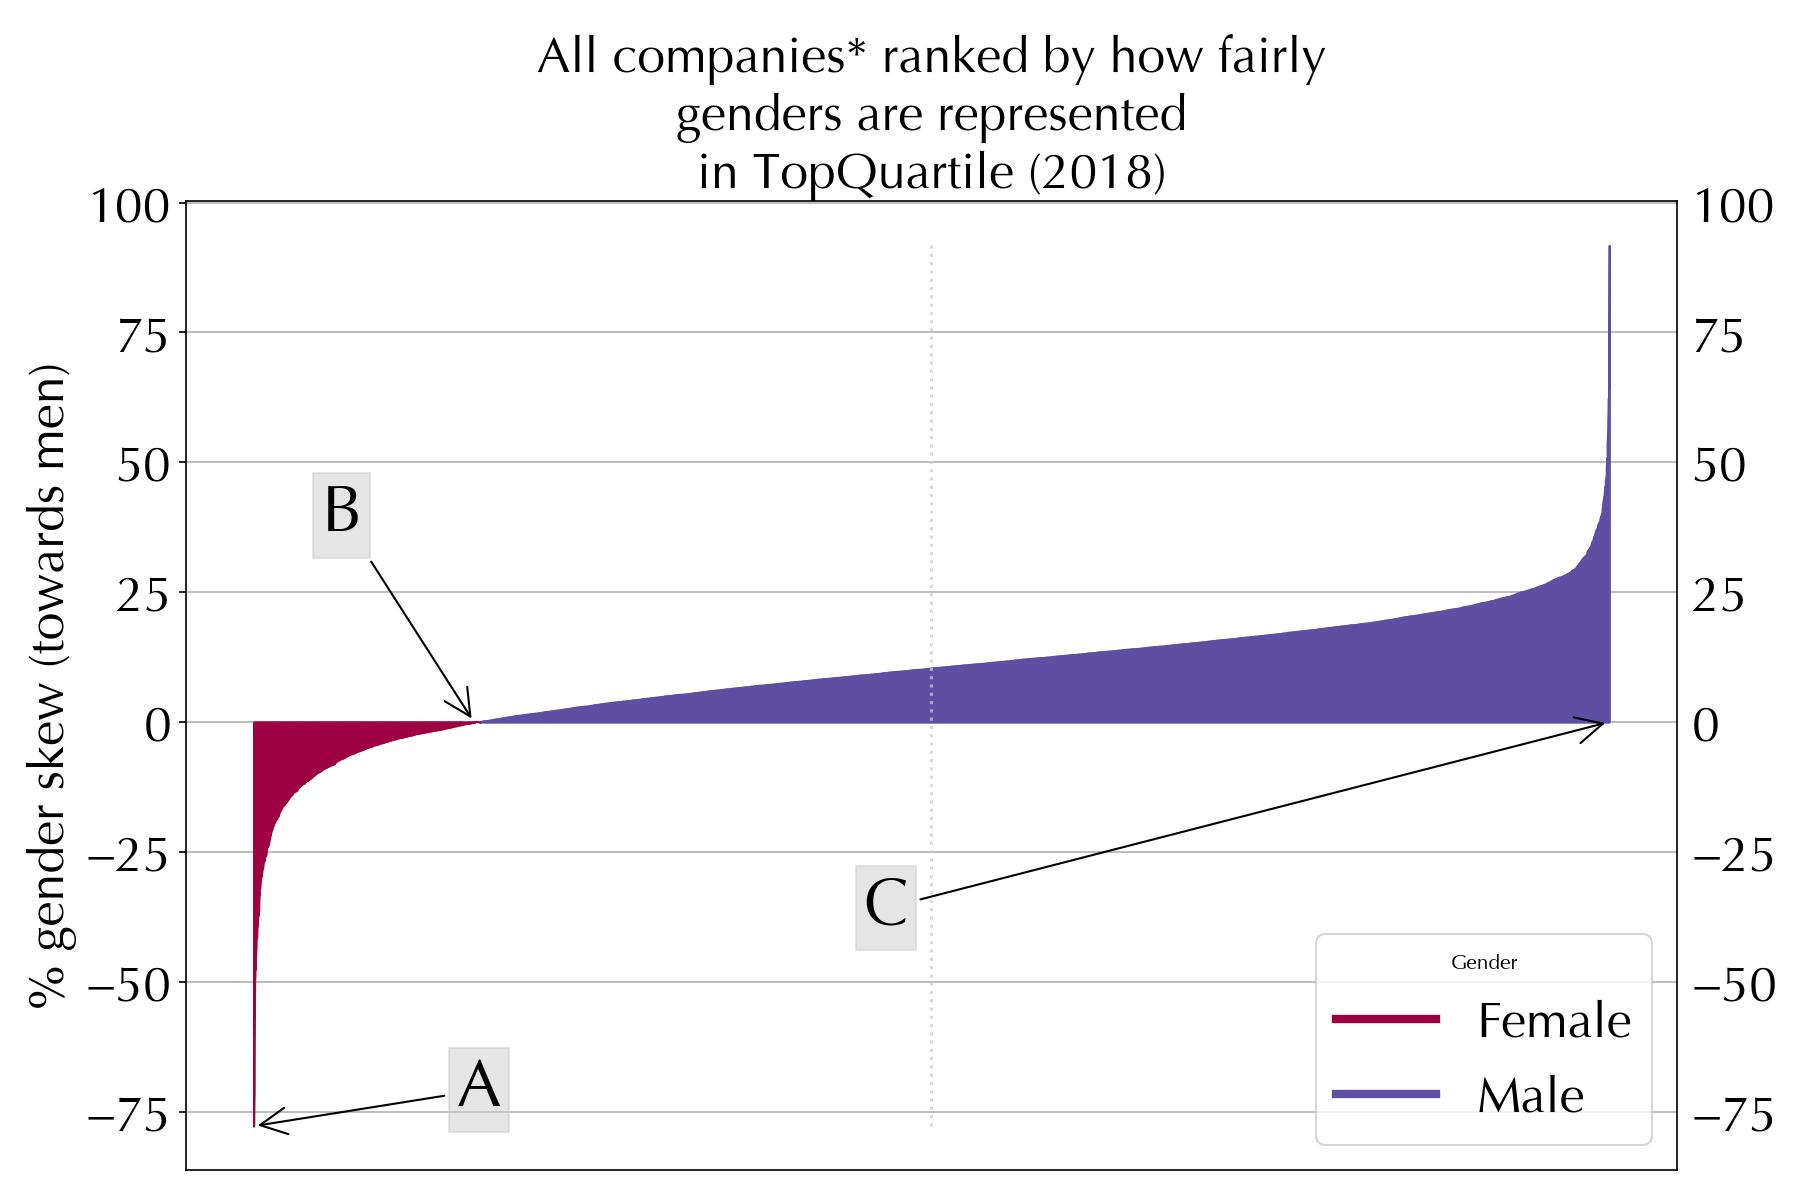
\includegraphics[width=\linewidth]{images/2018-how-fair-genders-TopQuartile.png}
        \captionof{figure}{            \begin{scriptsize} 
2018 Top quartile gender representation imbalance (only showing companies that had employees of both genders.) Companies are ranked by fairness of representation of gender in the quartile from most skewed towards women to most skewed towards men from left to right. \textbf{(A):} Most skewed towards women. At \emph{G. Burley \& Sons Limited} 100\% of the company's female employees
            are in the top quartile vs 22.2\% of the company's men. 3.6\% of employees are female. 
            \textbf{(B):} Most equal. At \emph{Newcross Healthcare Solutions Limited} 25\% of the company's women are in the top quartile vs 25\% of the company's men. 78.0\% of employees are female.
            \textbf{(C):} Most skewed towards men. At \emph{Randstad HR Solutions Limited} 4.8\% of the women
            employees are in the top quartile vs 96.6\% of the company's men. 78\% of the employees are
            female.        \end{scriptsize}}

        
        \label{fig:upper-quartile}
    \end{centering}
    
%%%%%%%%%%%%%%%%%%%%%%%%%%%%%%%%%%%%%%%%%%%%%%%%%%%%%%%%%%%%    
